\providecommand{\atd}{..}
\documentclass[../ATD.tex]{subfiles}
\usepackage{graphicx}

\begin{document}
    \chapter{Testing}\label{ch:testing}
    \section{Important note}\label{sec:important-note}
    An important issue has to be at least presented before to start to talk about the testing, since it compromises the correct use of the application.
    The issue will be discuss later, but it has a big impact on the structure of the document.
    \newline
    When the application run, after the user login an error message is show, and almost all the functionality of the application are not available.
    The error shows up on every device we used to run the application: web page (Chrome, as indicated), android phone, iOS phone, iOS simulator.
    We think that this issue cause the most of the fail on the test that will be presented in the next chapter.
    In the following are showed some picture of the error.
    \begin{figure}[H]
        \centering
        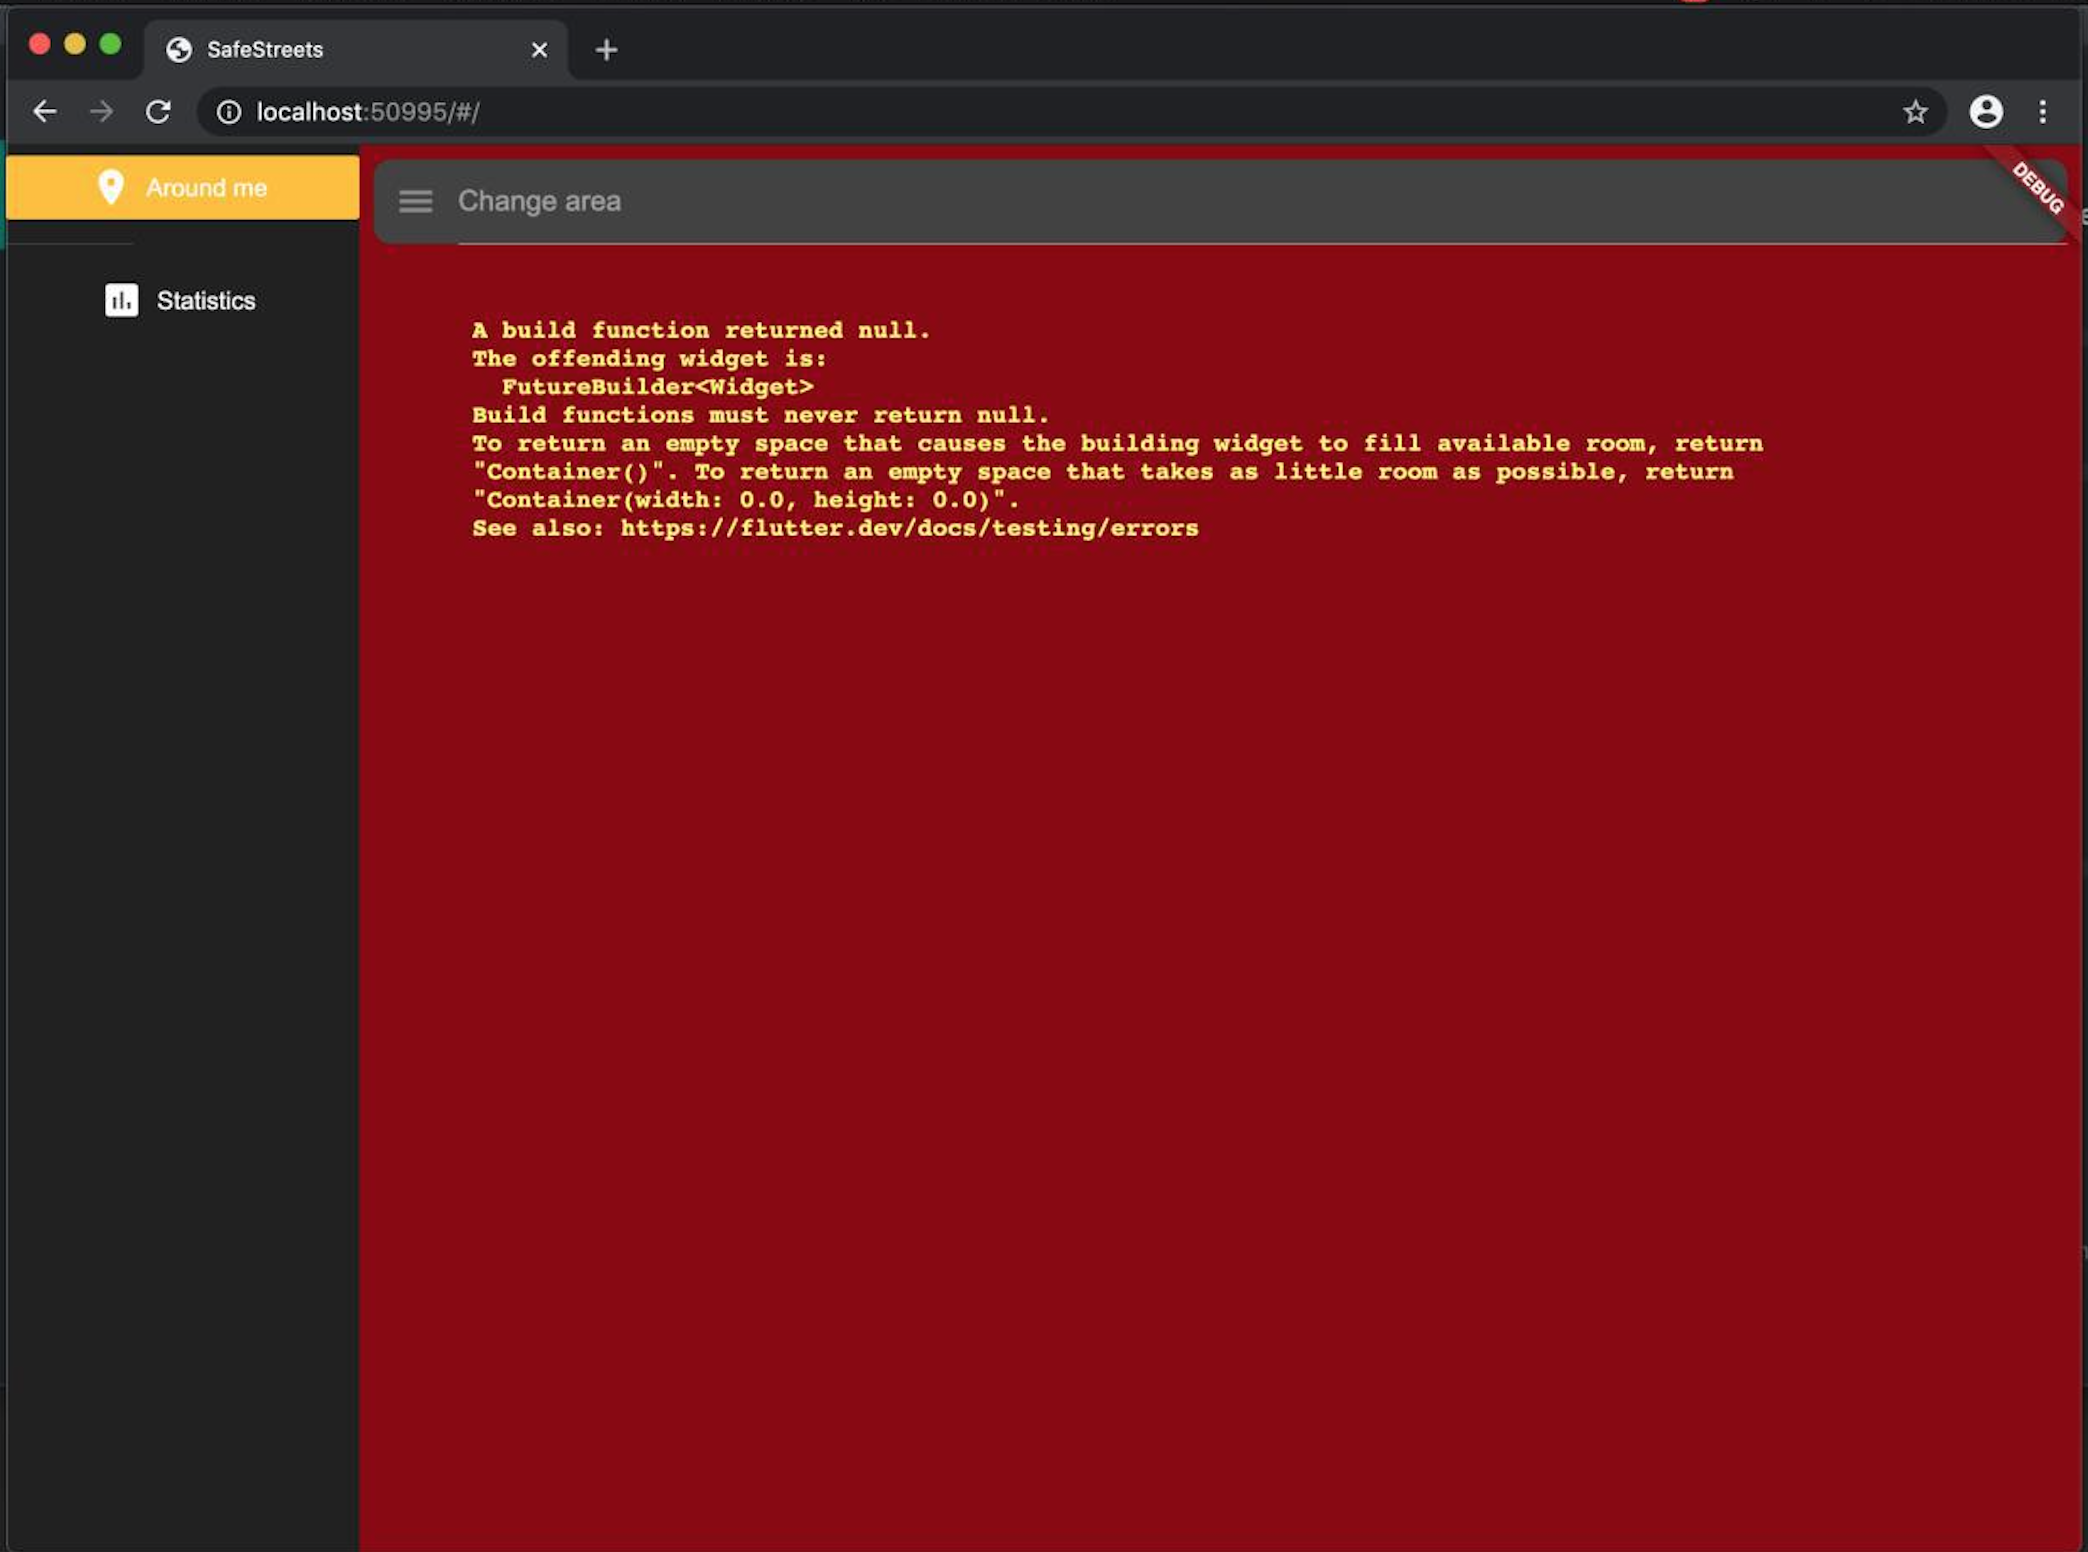
\includegraphics{../assets/web_page_error.png}
        \caption{Web page error}
    \end{figure}
    \begin{figure}[H]
        \centering
        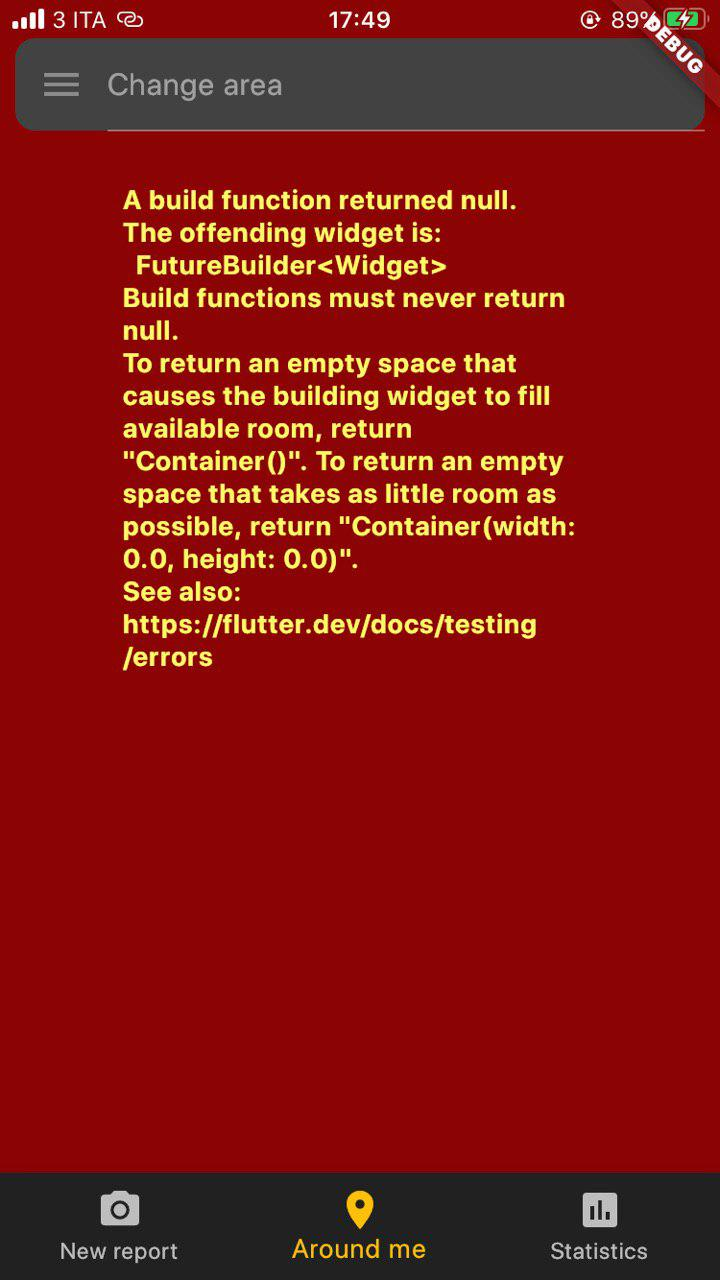
\includegraphics{../assets/smartphone_error.png}
        \caption{Smartphone error}
    \end{figure}
    \begin{figure}[H]
        \centering
        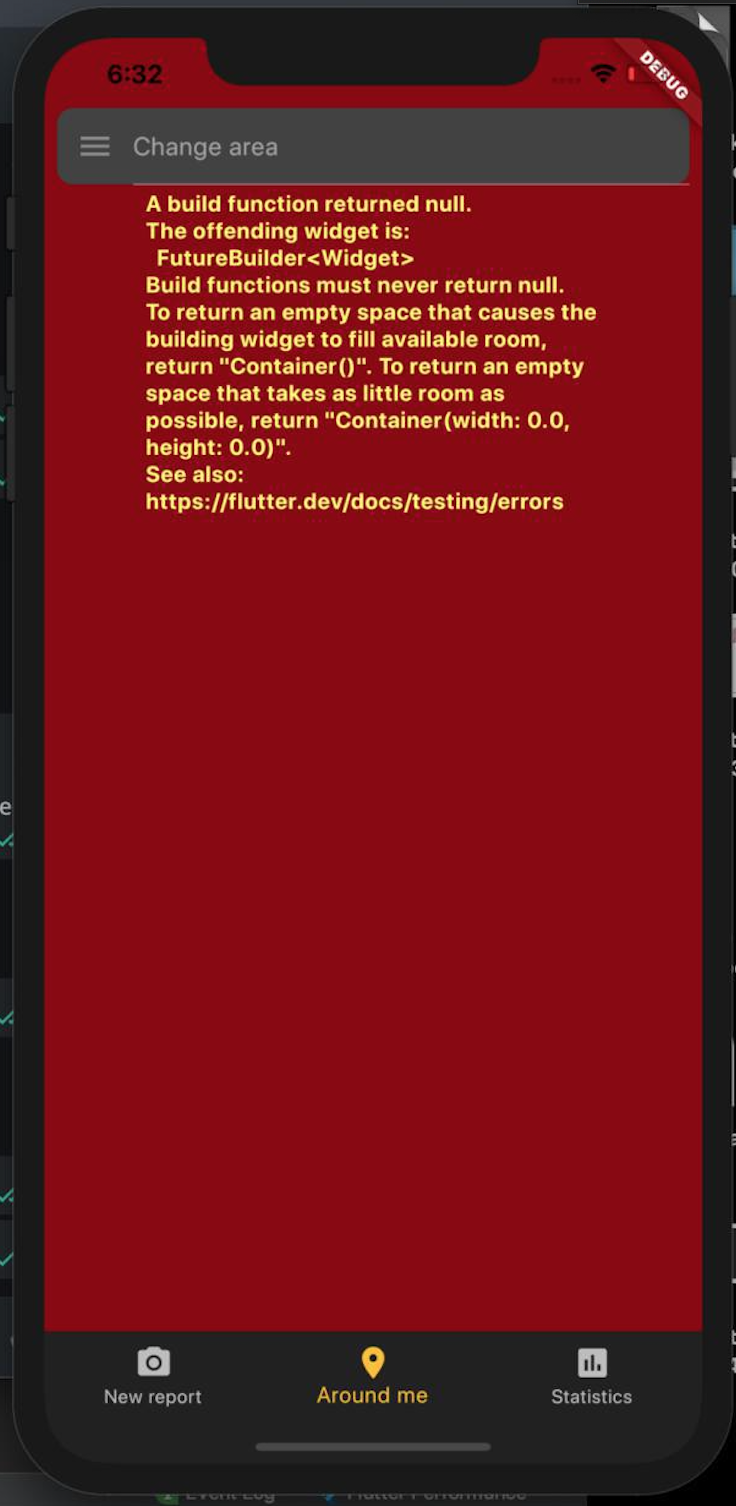
\includegraphics{../assets/iOS_simulator_error.png}
        \caption{iOS simulator error}
    \end{figure}

    \section{Testing Requirements Table}\label{sec:testing-requirements-table}
    Probably because of the already showed error, it will not be possible to test all the requirements since some of them will not be showed at all.
    Moreover, it will be difficult to follow the requirement order presented in the RASD and in the ITD while testing, so the following table purpose is to show which requirements will be tested.
    At the end of the chapter a section for the untested requirements will be provided anyway.

    ******** TABELLA *********

    \section{Test Cases}\label{sec:test-cases}
    The test cases will be presented as follow: they will be group by tested requirements, and for every test will be described the following information:
    \begin{enumerate}
        \item \textbf{Test purpose}
        \item \textbf{Device}: device on which the test run (android phone, iOS phone, simulator, web page, etc..)
        \item \textbf{Input}: input of the test
        \item \textbf{Outcome}: output of the test
        \item \textbf{Result}: passed or fail
        \item (Eventually) \testbf{Possible bugs}: list of possible bugs
        \item (Eventually) \textbf{Comment}: relevant comments about the test
    \end{enumerate}
    As previously explained, it will not be possible to test the requirements in the same order as they are presented in the RASD and ITD,
    but they will be marked with the same enumeration to make them easier to read.
    The requirements will be marked \textbf{[Rn]}, to refer to the n-th requirement.

    \subsection{User registration and login [R14]}\label{subsec:user-registration-and-login}
    R14: The system must allow the user to perform the registration and the login.

    \subsubsection{User login 1}\label{subsubsec:user-login-1}
    \begin{itemize}
        \item \textbf{Test purpose}: An user that is already signed in must be able to login correctly.
        \item \textbf{Device}: iPhone
        \item \textbf{Input}: username: "jak4", password: "jak".
        \item \textbf{Outcome}: SafeStreet user's main menu.
        \item \textbf{Result}: Passed
        \item \textbf{Comment}: The user "jak4" was already registered with the password "jak".
    \end{itemize}

    \subsubsection{User login 2}\label{subsubsec:user-login-2}
    \begin{itemize}
        \item \textbf{Test purpose}: An user that is already signed in must be able to login correctly.
        \item \textbf{Device}: web page
        \item \textbf{Input}: username: "jak4", password: "jak".
        \item \textbf{Outcome}: SafeStreet user's main menu.
        \item \textbf{Result}: Passed
        \item \textbf{Comment}: The user "jak4" was already registered with the password "jak".
    \end{itemize}

    \subsubsection{User login 3}\label{subsubsec:user-login-3}
    \begin{itemize}
        \item \textbf{Test purpose}: An user that is already signed in must be able to login correctly if the server is up.
        \item \textbf{Device}: iOS simulator
        \item \textbf{Input}: Server turned off, username: "jak4", password: "jak".
        \item \textbf{Outcome}: Nothing happen.
        \item \textbf{Result}: Passed
        \item \textbf{Comment}: Since the server is down, it is fine that nothing happen if i try to login.
    \end{itemize}

    \subsubsection{User login 4}\label{subsubsec:user-login-4}
    \begin{itemize}
        \item \textbf{Test purpose}: An user can not login with an unregistered account.
        \item \textbf{Device}: iOS simulator
        \item \textbf{Input}: username: "fakeTestAccount", password: "psw".
        \item \textbf{Outcome}: Invalid data message.
        \item \textbf{Result}: Passed
    \end{itemize}

    \subsubsection{User registration 1}\label{subsubsec:user-registration-1}
    \begin{itemize}
        \item \textbf{Test purpose}: An user must be allowed to register.
        The user try to register by providing all the information required.
        \item \textbf{Device}: iOS simulator
        \item \textbf{Input}: username: "test1", email: "test@test.it", name: "TestName", surname: "TestSurname", place of birth: "TestPlace", date of birth: "01-01-1001", place of residence: "TestPlace", fiscal code: "aaaaaaaaaaaaaaaa", password "testpsw", id photo: a picture from device, your photo: a picture from device
        \item \textbf{Outcome}: Nothing happen
        \item \textbf{Result}: Failed
        \item \testbf{Possible bugs}: The application does not perform any action, but on the intelliJ console it is possible to see an error "Unhandled Exception: FormatException: Invalid date format".
        \item \textbf{Comment}: Talking with the developer group, we know that the correct format for the date is yyyy-mm-dd.
        The application should inform the user about that restriction.
        Moreover, the application should show an error to inform the user that something went wrong, because it is not intuitive to understand that the sign up request has been sent.
    \end{itemize}

    \subsubsection{User registration 2}\label{subsubsec:user-registration-2}
    \begin{itemize}
        \item \textbf{Test purpose}: An user must be allowed to register.
        The user try to register by not giving any information.
        \item \textbf{Device}: iOS simulator
        \item \textbf{Input}: none
        \item \textbf{Outcome}: All the textual textfield are signed as mandatory.
        \item \textbf{Result}: Passed
        \item \textbf{Comment}: The "ID PHOTO" and "YOUR PHOTO" button are not marked as mandatory.
    \end{itemize}

    \subsubsection{User registration 3}\label{subsubsec:user-registration-3}
    \begin{itemize}
        \item \textbf{Test purpose}: An user must be allowed to register.
        The user try to register by giving all the information, except for the two pictures.
        \item \textbf{Device}: iOS simulator
        \item \textbf{Input}: username: "test1", email: "test@test.it", name: "TestName", surname: "TestSurname", place of birth: "TestPlace", date of birth: "1001-01-01", place of residence: "TestPlace", fiscal code: "aaaaaaaaaaaaaaaa", password "testpsw"
        \item \textbf{Outcome}: Nothing happen
        \item \textbf{Result}: Failed
        \item \textbf{Comment}: Nothing happen, but from the intelliJ console it is possible to see that the pictures are mandatory for the registration.
        They should be marked as mandatory as well as all the other fields, since it is not intuitive to understand what is going wrong.
    \end{itemize}

    \subsubsection{User registration 4}\label{subsubsec:user-registration-4}
    \begin{itemize}
        \item \textbf{Test purpose}: An user must be allowed to register.
        The user try to register by giving all the correct information.
        \item \textbf{Device}: iOS simulator
        \item \textbf{Input}: username: "test1", email: "test@test.it", name: "TestName", surname: "TestSurname", place of birth: "TestPlace", date of birth: "1001-01-01", place of residence: "TestPlace", fiscal code: "aaaaaaaaaaaaaaaa", password "testpsw", id photo: a picture from device, your photo: a picture from device
        \item \textbf{Outcome}: All the textual textfield are signed as mandatory.
        \item \textbf{Result}: Passed
        \item \textbf{Comment}: The "ID PHOTO" and "YOUR PHOTO" button are not marked as mandatory.
    \end{itemize}

    \subsubsection{User registration 5}\label{subsubsec:user-registration-5}
    \begin{itemize}
        \item \textbf{Test purpose}: An user must be allowed to register.
        The user try to register by giving all the correct information.
        \item \textbf{Device}: Web page (MacBook pro)
        \item \textbf{Input}: username: "test1", email: "test@test.it", name: "TestName", surname: "TestSurname", place of birth: "TestPlace", date of birth: "1001-01-01", place of residence: "TestPlace", fiscal code: "aaaaaaaaaaaaaaaa", password "testpsw"
        \item \textbf{Outcome}: The web page do not open neither the camera or the gallery.
        \item \textbf{Result}: Failed
        \item \textbf{Comment}: Since neither the camera or the gallery can be used to upload a picture, the registration can not be performed by the web page (the pictures are mandatory information for the registration).
    \end{itemize}

    \subsubsection{User registration 6}\label{subsubsec:user-registration-6}
    \begin{itemize}
        \item \textbf{Test purpose}: An user must be allowed to register.
        The user try to register by giving all the correct information.
        \item \textbf{Device}: iPhone
        \item \textbf{Input}: username: "federico111", email: "federico.innocente.spam@gmail.com", name: "Federico", surname: "Innocente", place of birth: "Pordenone", date of birth: "1997-06-19", place of residence: "Pordenone", fiscal code: "NNCFRC97H19G888Q", password "passwordP1", id picture: picture from camera, your picture: picture from camera.
        \item \textbf{Outcome}: Nothing happen
        \item \textbf{Result}: Failed
        \item \textbf{Comment}: I can assume that the registration failed, since I provided all real information and if I try to go back in sign in page and log in, a message said that I am using invalid email and password.
    \end{itemize}

    \subsection{Municipality registration and login [R15]}\label{subsec:municipality-registration-and-login}
    R15: The system must allow the Municipality to perform the registration and the login.

    \subsubsection{Municipality login 1}\label{subsubsec:municipality-login-1}
    \begin{itemize}
        \item \textbf{Test purpose}: A municipality that is already signed in must be able to login correctly.
        \item \textbf{Device}: iOS simulator
        \item \textbf{Input}: username: "Milano", password: "Milan".
        \item \textbf{Outcome}: SafeStreet municipality's main menu.
        \item \textbf{Result}: Passed
        \item \textbf{Comment}: The municipality "Milano" was already registered with the password "Milan".
    \end{itemize}

    \subsubsection{Municipality login 2}\label{subsubsec:municipality-login-2}
    \begin{itemize}
        \item \textbf{Test purpose}: An user that is already signed in must be able to login correctly.
        \item \textbf{Device}: Web page
        \item \textbf{Input}: username: "Milano", password: "Milan".
        \item \textbf{Outcome}: SafeStreet municipality's main menu.
        \item \textbf{Result}: Passed
        \item \textbf{Comment}: The user "Milano" was already registered with the password "Milan".
    \end{itemize}

    \subsubsection{Municipality registration}\label{subsubsec:municipality-registration}
    \begin{itemize}
        \item \textbf{Test purpose}: A municipality must be able to register itself on SafeStreets.
        \item \textbf{Device}: Web page (MacBook pro)
        \item \textbf{Input}: activation code: "123123123", username: "Test", password: "TestPsw".
        \item \textbf{Outcome}: Nothing happen.
        \item \textbf{Result}: Failed
    \end{itemize}

    \subsection{Picture selection [R8]}\label{subsec:picture-selection}
    R8: The system must allow the User to take a picture or select one from the device.
    This requirement must be ensured in two cases: when a user upload pictures for the registration and when the user upload pictures for a violation.

    \subsubsection{Picture selection for registration 1}\label{subsubsec:picture-selection-for-registration-1}
    \begin{itemize}
        \item \textbf{Test purpose}: A user must be allow to take a picture or to select one from the device when he want to register himself.
        \item \textbf{Device}: iPhone
        \item \textbf{Input}: "Chose ID photo" button from the sign in page.
        \item \textbf{Outcome}: A choice is given to the user between using his camera or selecting from gallery.
        Both the options work properly.
        \item \textbf{Result}: Passed
        \item \textbf{Comment}: The same operation can be done for the "Chose your photo" button, with the same result.
        After selecting a picture, nothing change on the application page, but this can be think as a choice and do not go against the requirement.
    \end{itemize}

    \subsubsection{Picture selection for registration 2}\label{subsubsec:picture-selection-for-registration-2}
    \begin{itemize}
        \item \textbf{Test purpose}: A user must be allow to take a picture or to select one from the device when he want to register himself.
        \item \textbf{Device}: Web App (MacBook pro)
        \item \textbf{Input}: "Chose ID photo" button from the sign in page.
        \item \textbf{Outcome}: A choice is given to the user between using his camera or selecting from gallery, but than nothing happen for both the choice.
        \item \textbf{Result}: Failed
        \item \textbf{Comment}: The same operation can be done for the "Chose your photo" button, with the same result.
    \end{itemize}

    \subsubsection{Picture selection for violation 1}\label{subsubsec:picture-selection-for-violation-1}
    \begin{itemize}
        \item \textbf{Test purpose}: A user must be allow to take a picture or to select one from the device when he want to upload pictures in the context of a violation.
        \item \textbf{Device}: iPhone
        \item \textbf{Input}: Tapping on "New Report" option from the main menu.
        \item \textbf{Outcome}: The camera is opened by default, but then it is possible to switch to the gallery to chose a picture.
        Both option allow you to select a picture and move to the next step a the violation reporting.
        \item \textbf{Result}: Passed
    \end{itemize}
    


\end{document}